\chapter{Background}
\label{chap:background}

    \section{Hardware Description}
    \label{sec:hardware-description}
        The hardware development process can be well understood by analyzing its
        similarities and differences to software development.
        Both hardware and software development usually "begin" with a high-level \emph{specification}
        of the algorithm to be implemented.
        Also, both proceed by a series of translations, increasingly adding more details to the description.

        However, the final targets of both hardware and software development differ:
        while in software the final artifact is machine code (sequence of instructions) for some architecture,
        in hardware the target is usually a \emph{floorplan}, a spacially placed graph of logic gates and wires.

        Also, the transformation steps in the software and hardware chains are different,
        as depicted in Figure~\ref{fig:sw-hw-chains}.
        In this figure, the rectangular boxes represent transformations steps towards a more detailed description,
        while the ellipsoid shapes represent artifacts that are consumed/produced by each step.

        \begin{figure}[ht]
            \centerline{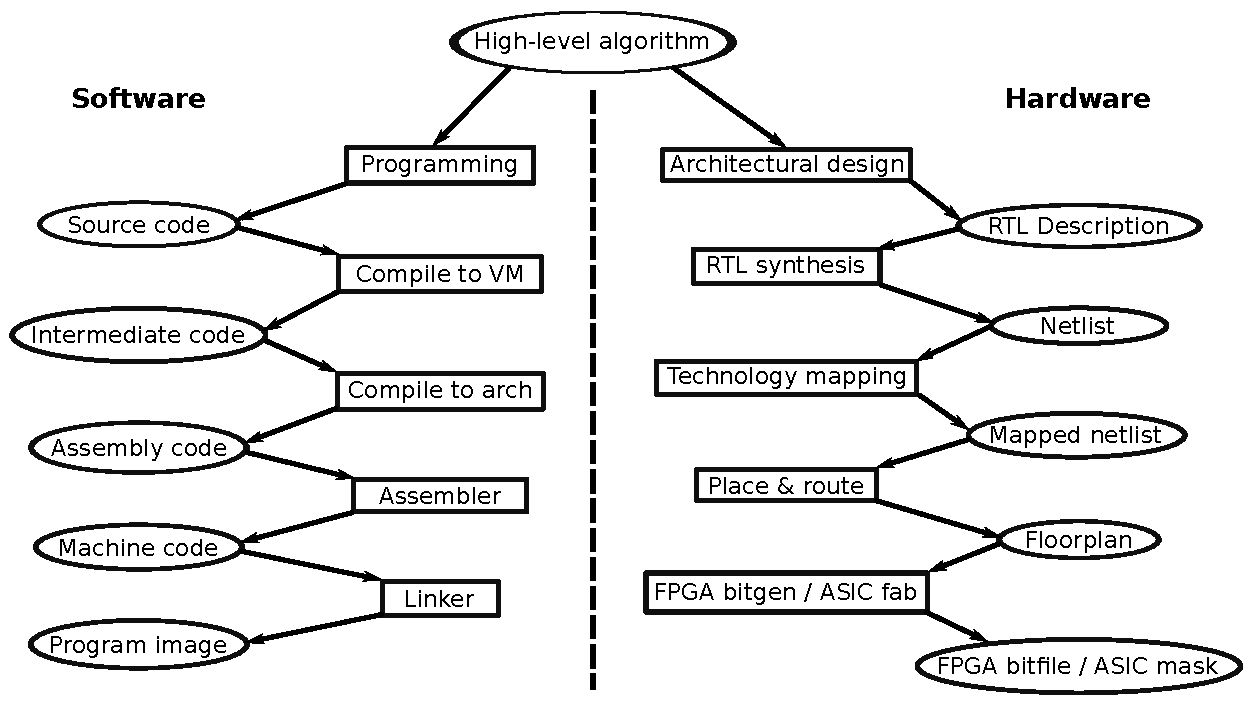
\includegraphics[width=1.0\textwidth]{imgs/sw-hw-chains.pdf}}
            \caption{Software and Hardware refinement chains. \label{fig:sw-hw-chains}}
        \end{figure}

        \acrodef{HDL}{Hardware Description Language}
        \acrodef{RTL}{Register-Transfer Level}
        The first (highest) two levels in the hardware implementation flow are usually described using
        so-called \acp{HDL}, usually Verilog or \acs{VHDL}.
        Nowadays they are used by hardware engineers to write both behavioural specifications of circuits
        (topmost ellipsis in Figure~\ref{fig:sw-hw-chains}) as well as \ac{RTL} descriptions.
        However, these languages were originally designed for \emph{simulation} purposes,
        and there are several problems that arise when using them to
        model hardware \emph{architecture} and behaviour.

        First of all, only a \emph{subset} of these languages can be used for \emph{synthesis}
        (actually deriving a netlist and floorplan).
        Although there is a standard~\cite{ieee1076-3-synth-vhdl} defining a \emph{synthesizable subset} of \acs{VHDL},
        tools differ greatly in the level of support.

        To further complicate the matter, this synthesizable subset is not \emph{syntactically seggregated}.
        One example of complex requirement for synthesizability of \acs{VHDL} is:
        "in a process, every output must be assigned a value for every possible combination of input values".
        In Listing~\ref{lst:vhdl-unsynth-process} we have an example process violating this requirement
        (the \texttt{if} statement lacks an \texttt{else} branch, and the \texttt{y} output has no assigned
        value when \texttt{sel} is different than zero).

        \begin{listing}[ht]
            \centering{\vhdlfile{code/vhdl/vhdl-unsynth-process.vhd}}
            \caption{Unsynthesizable \acs{VHDL} process.\label{lst:vhdl-unsynth-process}}
        \end{listing}

        Another significant difference between hardware and software development
        is the level of \emph{automatization} in the chains (Figure~\ref{fig:sw-hw-chains}).
        Usually, all transformation steps in the software chain are automatic.
        On the hardware chain, the \emph{crucial} "Architectural design" step is mostly manual.

        The complex task of making explicit the space-time trade-offs lays in the hands of the hardware designer:
        they must decide how much parallelism to use, how to pipeline the processing steps of the algorithm,
        taking care to not generate data hazards, etc.

        \acrodef{HLS}{High-Level Synthesis}
        Recently, tools have been developed for this first step – called \ac{HLS}.
        They usually take \emph{behavioural \acs{VHDL}}, C or even C++ as input, and produce \ac{RTL} code.
        However, current \acs{HLS}-based hardware implementation chains still face two main problems:

        \begin{itemize}
            \item The input languages (VHDL, C) are not expressive enough.
            \item Specification, verification and synthesis are all done with different tools and different languages.
            \begin{itemize}
                \item Even behavioural \acs{VHDL} can be considered practically a different language
                    than \acl{RTL} \acs{VHDL}.
            \end{itemize}
        \end{itemize}

        Functional programming languages have been touted as a solution to both of these problems.
        A functional program is a more abstract and expressive specification of an algorithm than
        a C function or VHDL entity.
        Also, functional languages could be used to \emph{both} write the specification of a circuit's behaviour,
        as well as its \acl{RTL} description.


    \section{Functional Hardware Description}
    \label{sec:functional-hardware}
        In the beginning of the 1980s, many researchers were trying to use functional programming languages
        to design and reason about hardware circuits.
        These developments were happening at the same time when the \ac{VHDL} was being designed and standardized.
        Even though \ac{VHDL} and Verilog ended up "winning" and becoming the \emph{de facto} industry standards,
        it is still useful to take a look at the ideas behind these early \acp{HDL}, as some of them
        inspired current approaches.

        The idea was then to come up with new functional languages, \emph{specialized} to do hardware description.
        One of the prominent early examples in this set is μFP~\cite{mufp-1984},
        which was in turn inspired by John Backus's FP~\cite{backus-turing-lecture}.
        In contrast to \ac{VHDL}, which was later adapted to synthesis in an ad-hoc way,
        μFP was designed since the beginning to have both interpretations:

        \begin{description}
            \item[Behavioural]
                Each "primitive" circuit as well as each combining form (higher-order function)
                has an attached \emph{functional semantics}, used in simulation.
            \item[Geometric]
                Each combining form has a typical geometric interpretation.
                For example, sequential composition of two circuits \AB{c₁} and \AB{c₂} will result
                in a floorplan in which \AB{c₂} is placed \emph{adjacent to} \AB{c₁} and connected to it
                by the required wires.
        \end{description}

        The μFP language is an \emph{extension} of Backus's FP, and contained only one extra combining form: μ.
        The μ combining form is responsible for the creation of functions (circuits) with internal state.
        According to the seminal μFP paper~\cite{mufp-1984}:

        \begin{quote}
            The meaning of μf is defined in terms of the meaning of f.
            The functional \texttt{out} hides the state
            so that while $M(f)$ maps a sequence of input-state pairs to a sequence of output-state pairs,
            $\text{out}(M(f))$ just maps a sequence of inputs to a sequence of outputs.
            For a given cycle, the next output and the next state depend on the current input and the current state.
        \end{quote}

        One very simple example of a circuit with internal state is a shift register.
        In Figure~\ref{fig:mufp-shift}, we can see the structure of this circuit.
        Each of the dotted boxes represents a μFP expression.
        The smaller box denotes a combinational circuit (with 2 inputs and 2 outputs) that swaps its inputs.
        The bigger box corresponds to the application of the μ combinator to the smaller one.
        It adds the indicated latch and a feedback loop, creating a stateful circuit.

        \begin{figure}[ht]
            \centerline{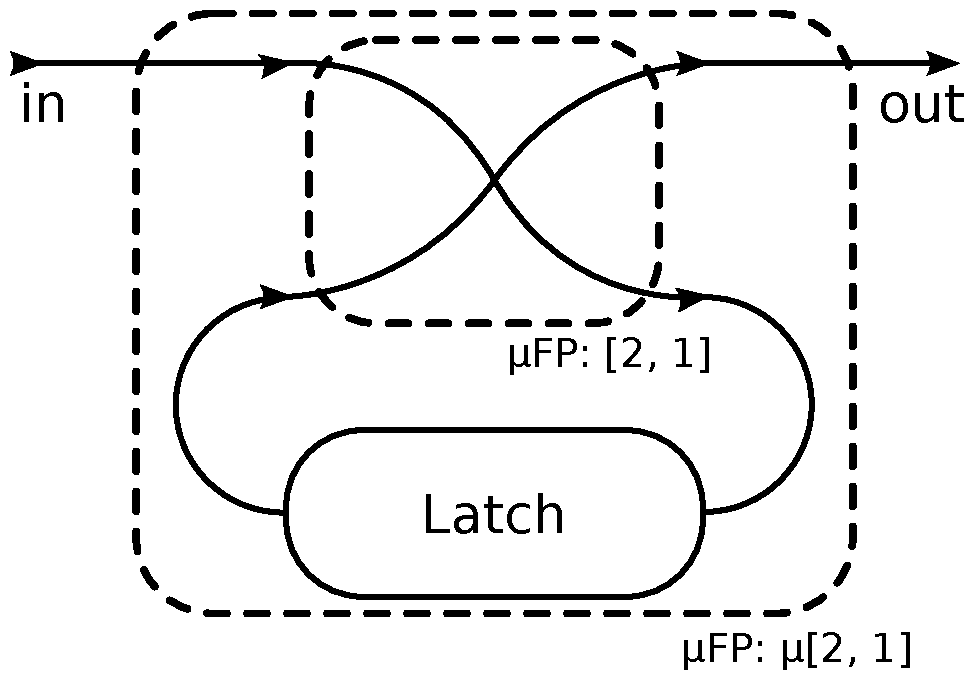
\includegraphics[width=0.5\textwidth]{imgs/mufp-shift.pdf}}
            \caption{\emph{Shift register}: a simple example of sequential circuit in μFP. \label{fig:mufp-shift}}
        \end{figure}

        By being a conservative extension of Backus's FP, almost all algebraic laws of FP also hold for μFP.
        Furthermore, the μ combining form has useful algebraic laws of its own.
        The most notable of these laws states that the composition of two "μ-wrapped" functions
        can be converted to a single "μ-wrapper".

        In other words: a circuit with several, localized, memory elements can be converted into a circuit
        with a single centralized memory bank and a combinational block.
        If we apply this rewrite rule from right to left, we can see it as a form of "optimization",
        in which we start with a single memory bank and refine the design towards one in which
        memory elements sit closer to the sub-circuits using them.

        Two of the core ideas of μFP served as inspiration for Π-Ware:

        \begin{description}
            \item[Double interpretation] As in μFP,
                each circuit and circuit combinator in Π-Ware has two distinct semantics:
                they can be simulated (functional semantics) or synthesized to a netlist (geometric semantics).
            \item[Single sequential constructor] As in μFP,
                there is only \emph{one way} in Π-Ware to construct a sequential circuit.
                Also, the same law regarding the \emph{state-introducing constructor} holds in Π-Ware,
                but because we use Agda as host language, this meta-theoretical property can be proven
                \emph{in the same language} in which circuits are described.
        \end{description}


        \subsection{Embedded Functional Hardware Description}
        \label{subsec:embedded-functional-hardware}
            \acrodef{EHDL}{Embedded Hardware Description Language}
            With the growing popularity and advocacy~\cite{hudak-edsls} of \emph{embedded} \acp{DSL},
            a trend emerged of also having embedded \acp{HDL}.
            Functional programming languages were a natural fit for hosting \acp{DSL}.
            In particular, the Haskell programming language proved to be a popular choice of host,
            due to features such as lazy evaluation and a highly-customizable syntax.

            Some examples of highly-successful \acp{DSL} implemented in Haskell are:

            \begin{itemize}
                \item Attoparsec~\footnote{\url{https://github.com/bos/attoparsec}} (monadic parsing)
                \item Accelerate~\footnote{\url{https://github.com/AccelerateHS/accelerate/wiki}} (data-parallel computing)
                \item Esqueleto~\footnote{\url{https://github.com/prowdsponsor/esqueleto}} (SQL queries)
                \item Diagrams~\footnote{\url{http://projects.haskell.org/diagrams/}} (2D and 3D vector graphics)
            \end{itemize}

            Also, some of the most popular and powerful \acp{EHDL} are hosted by Haskell.
            Let us now present some of these \acp{EHDL} and discuss some of their limitations,
            which will lead to the question of how to solve them using dependent types.

            \subsubsection{Lava}
            Perhaps the most popular family of hardware \acp{DSL} embedded in Haskell is the \emph{Lava} family.
            Lava's first incarnation~\cite{lava-1999} was developed at Chalmers University of Technology
            and Xilinx, and used a shallow-embedding in Haskell, along with a monadic description style
            to handle naming and sharing.
            These circuit monads were parameterized, and by using different instances,
            different interpretations could be given to a single circuit description, such as
            simulation, synthesis, or model checking.

            The design of Lava suffered significant changes later on, abandoning the monadic interface
            and adopting an observable sharing solution based on reference equality~\cite{observable-sharing-circuits}.
            Currently, Lava has several dialects, such as \emph{Chalmers-Lava}, \emph{Xilinx-Lava}, \emph{York-Lava} and \emph{Kansas-Lava}.
            We base our examples in \emph{Chalmers-Lava}~\footnote{\url{https://hackage.haskell.org/package/chalmers-lava2000}},
            which can be said to be the "canonical" dialect, and also the most actively developed.

            In Lava, circuits are written as normal Haskell functions, by using pattern matching,
            function application and local naming.
            One restriction is that the types of the arguments are
            constructed by the \texttt{Signal} type constructor.
            For example, a negation gate in Lava would have the following type signature:

            \begin{haskellcode}
        inv :: Signal Bool -> Signal Bool
            \end{haskellcode}

            Another restriction is that all circuit inputs must be \emph{uncurried}, i.e.,
            even though the \emph{circuit} has several inputs, the \emph{function} modeling that circuit
            must have only one argument, with all inputs in a \emph{tuple}.
            A \texttt{NAND} gate in Lava would look like this:

            \begin{haskellcode}
        nand2 :: (Signal Bool, Signal Bool) -> Signal Bool
        nand2 (a, b) = inv (and2 (a, b))
            \end{haskellcode}

            Finally, due to the instances provided for the \texttt{Signal} type, the only way to
            aggregate bits in Lava is by using tuples and lists.
            Using only these structures we forego some type safety that Haskell \emph{could} provide.
            For example, an n-bit binary (ripple-carry) adder in Lava has the following description:

            \begin{haskellcode}
        adder :: (Signal Bool, ([Signal Bool], [Signal Bool]))
              -> ([Signal Bool], Signal Bool)

        adder (carryIn, ([] ,[]))    = ([], carryIn)
        adder (carryIn, (a:as, b:bs) = (sum:sums, carryOut)
            where (sum, carry)     = fullAdd (carryIn, (a, b))
                  (sums, carryOut) = adder (carry, (as, bs))
            \end{haskellcode}

            In this circuit description, there is an \emph{expectation} that both inputs have the same size.
            When this expectation is not met, a \emph{run-time} error will occur during simulation.
            This happens because the given definition is \emph{partial}:
            the cases for \texttt{(carryIn, ([], b:bs))} and \texttt{(carryIn, (a:as, []))} are left undefined.

            This limitation of Lava can be solved by dependent types, namely by using statically-sized vectors.
            Another limitation of Lava is related to the way in which it solves the observable sharing question:
            in order to detect sharing and cycles, the equality over the \texttt{Signal} type is defined
            as an equality over the references used.
            Therefore, comparisons of signals "created" in different sites will fail,
            even though their values are the same.
            For example, the following expressions will evaluate to \texttt{False}:

            \begin{haskellcode}
        test1 :: Bool
        test1 = low == low

        test2 :: Bool
        test2 = simulate adder (low, ([low], [low])) == low
            \end{haskellcode}

            This limitation is also not present in Π-Ware, due to the way in which we describe circuits
            in a structural fashion, completely avoiding the need to deal with observable sharing.


            \subsubsection{ForSyDe}
            Another example of \ac{EHDL} in Haskell is ForSyDe~\cite{forsyde1999}.
            ForSyDe and Lava differ substantially in description style and internal workings,
            and a more complete comparison of the two can be found
            in the final report~\cite{functional-hardware-survey}
            of the experimentation project conducted as preparation to this thesis.

            In ForSyDe, the central concepts are those of \emph{process} and \emph{signal}.
            Whereas in Lava only \emph{synchronous} sequential circuits can be described – that is
            also the case in Π-Ware – in ForSyDe processes can belong to synchronous,
            asynchronous and continuous \emph{models of computation}.

            In the synchronous model of computation (which we studied more deeply),
            process constructors take a combinational function (called \emph{process function} in
            ForSyDe jargon) and turn it into a synchronous sequential circuit
            (for example a state machine).

            \acrodef{AST}{Abstract Syntax Tree}
            Instead of just using (smart) constructors of a certain \emph{circuit datatype} to build
            process functions, ForSyDe relies on \emph{Template Haskell} to
            \emph{quote} regular Haskell syntax into an \ac{AST} – which is then further processed by ForSyDe.
            For example, the description of an adder in ForSyDe would look like the following:

            \begin{haskellcode}
        adderFun :: ProcFun (Int8 -> Int8 -> Int8)
        adderFun = $(newProcFun [d|
                adderFun' :: Int8 -> Int8 -> Int8
                adderFun' x y = x + y
            |])

        adderProc :: Signal Int8 -> Signal Int8 -> Signal Int8
        adderProc = zipWithSY "adderProcess" adderFun
            \end{haskellcode}

            Notice how the \texttt{adderFun} \emph{process function} is built from a regular Haskell function
            (\texttt{adderFun'}), which is then \emph{quoted} (by the \texttt{[d|} quasi-quoter), processed by
            \texttt{newProcFun} and finally \emph{spliced} back into place.
            The (combinational) process function is then \emph{lifted} into the synchronous sequential setting
            by the \texttt{zipWithSY} \emph{process constructor}, which just "zips" the inputs signals (streams)
            by applying the given process function \emph{pointwise}.

            Not any Haskell function can be quoted and processed by \texttt{newProcFun}
            and turned into a ForSyDe process function: the argument and return types of a \texttt{ProcType}
            must belong to the \texttt{ProcType} type class. Instances of this class are provided only for:

            \begin{description}
                \item[Primitive types] \texttt{Int}, \texttt{Int8}, \texttt{Int16}, \texttt{Int32}, \texttt{Bool}, \texttt{Bit}
                \item[Enumerated types] User-defined enumerations, with derived instances for \texttt{Data} and \texttt{Lift}
                \item[Containers] Tuples and fixed-length vectors (\texttt{Data.Param.FSVec}),
                    holding a type of the above two categories and unrestrictedly nested.
            \end{description}

            Under certain conditions, ForSyDe is able to generate \ac{VHDL} netlists from the system description.
            In order for a ForSyDe system description to be \emph{synthesizable},
            all \emph{process functions} need to comply with some extra requirements:

            \begin{description}
                \item[Pointed notation] Declarations with point-free notation are not accepted
                \item[Single-clause] To be synthesizable,
                    the body of a \emph{process function} cannot have multiple clauses,
                    and it cannot have \texttt{let} or \texttt{where} blocks.
                    This essentially forbids recursion inside \emph{process functions}.
                    Pattern matching is only possible by using the \texttt{case} construct.
            \end{description}

            Despite all these limitations,
            ForSyDe still provides a more typed approach to hardware description than Lava,
            with perhaps its most distinctive feature being the usage of fixed-length vectors.
            In the \texttt{parameterized-data} package page
            on \emph{Hackage}~\footnote{\url{http://hackage.haskell.org/package/parameterized-data-0.1.5}},
            the authors admit that the library's function is to provide
            "type-level computations and \emph{emulate dependent types}".
            Therefore it is not a stretch to assume that using \emph{actual} dependent types
            could improve on the ideas proposed by ForSyDe.


            \subsubsection{Hawk and Cλash}
            Finally, in this short review of functional hardware \acp{EDSL},
            there are two more alternatives to be mentioned: Hawk and Cλash.

            Hawk~\cite{hawk-haskell} is a Haskell-hosted \ac{EDSL} with a different target than
            the ones presented until now: instead of modelling circuits, it intends to model \emph{microarchitectures}.
            Therefore, it has a higher level of abstraction than Lava or even ForSyDe.

            Models in Hawk are executable, and \emph{shallow-embedded}.
            However, Hawk uses a technique similar to the original Lava version~\cite{lava-1999}
            in order to also allow for symbolic evaluations:
            The descriptions are "parameterized" by type classes
            (in Hawk's case they are \texttt{Instruction}, \texttt{Boolean}, etc.),
            and by providing different instances, different \emph{interpretations} are achieved.

            The authors of Hawk mention some shortcomings of Haskell which they met, among which:

            \begin{itemize}
                \item Haskell's \texttt{List} datatype doesn't quite match
                    the intended semantics for Hawk's \texttt{Signals}:
                    the preferred semantics for \texttt{Signal} should be a truly infinite, coinductive \emph{stream}.
                    The authors mention a parallel effort of them to embed Hawk in the Isabelle theorem prover,
                    which achieved the desired semantics.
                    In Π-Ware, we make use of \emph{coinductive streams}~\cite{introduction-coalgebra-jacobs}
                    to model the inputs and outputs of synchronous sequential circuits,
                    exactly as the authors of Hawk desired.
                \item The type class system of Haskell is limited: the authors mention the desire to be able
                    to explicitly provided specific instances at specific sites,
                    and also the desire to use \emph{views} on datatypes.
                    Both features are available on \emph{Agda}.
            \end{itemize}

            Finally, we would like to mention Cλash~\cite{clash-baaij}.
            Even though it is not (strictly speaking) an \emph{embedded} \ac{DSL},
            it has very powerful features.

            Cλash was developed at the University of Twente,
            as an independent \ac{DSL}, i.e, with a compiler of its own.
            However, its source language is strongly based on Haskell, and Cλash's compiler
            reuses several pieces of machinery from Haskell's toolchain (specifically, GHC),
            in order to perform its term-rewriting and supercompilation.

            The circuit models in Cλash are higher-order, polymorphic functional programs,
            and they can be synthesized to \ac{VHDL} netlist.
            In this sense, Cλash serves as a good \emph{target} with which to compare hardware
            \ac{EDSL} development efforts: it is not – in itself – embedded, but has the same goals.


    \section{Dependently-Typed Programming}
    \label{sec:dtp}

        \subsection{Type systems}
        \label{subsec:type-systems}
            A type system, in the context of programming languages,
            serves the purpose of grouping values, so that meaningless and potentially undesirable operations are avoided.
            For example, in some dynamic languages, a string and an integer can be "added",
            because the language runtime first \emph{implicitly casts} the integer to a string,
            effectively performing string concatenation.
            This \emph{implicit} behaviour can cause all sorts of programmer mistakes to go undetected.
            It is also hard to formulate properties about addition \emph{in general} when all sorts
            of coercions can happen at runtime.
            To define addition sensibly, therefore, a type system can help by
            banning all programs that would try to add incompatible values.

            Type systems can have very different properties and be implemented in very different ways.
            Some of the ways in which type systems can be categorized are~\cite{understanding-types-cardelli}:

            \begin{itemize}
                \item Weak vs. strong
                \item Static vs. dynamic
                \item Polymorphism (parametric, ad-hoc, subtyping)
            \end{itemize}

            The most basic form of abstraction – values depending on values (the concept of functions) – is
            supported in practically all type systems.
            In some systems, the result type of functions can also depend on the \emph{types} of the arguments;
            this property is called \emph{polymorphism}.
            There are two kinds of polymorphism relevant to our discussion:

            \begin{itemize}
                \item In \emph{parametric polymorphism}, functions are written without mentioning any specific type,
                    and can therefore be applied to any instantiation of the type variable.
                    A typical example of a parametric polymorphic function is obtaining the length of a list,
                    where the same definition works for any type of element in the list.

                \item In \emph{ad-hoc polymorphism}, the behaviour of a function varies with the type of the inputs.
                    In Haskell, ad-hoc polymorphism is implemented in the \emph{type class system}.
                    A typical example of an ad-hoc polymorphic function is a comparison-based sorting algorithm
                    in which – depending on the type of the elements in the collection – different
                    comparison operators are be used.
            \end{itemize}

            Polymorphism adds \emph{expressivity} and makes a type system stronger,
            in the sense that it allows for more precise specifications.
            For example, if we want to implement a \texttt{swap} function for pairs in Haskell,
            we could do start by specifying the type of the function in a non-polymorphic way:
            \begin{haskellcode}
        swap' :: (Int , Int) -> (Int , Int)
            \end{haskellcode}

            There are several definitions satisfying the above type which do not swap the elements.
            For example, one "wrong" implementation would output a constant pair:
            \begin{haskellcode}
        swap' _ = (1 , 1)
            \end{haskellcode}

            Notice how the argument is ignored (we use the "don't care" pattern).
            To \emph{rule out} this class of wrong implementations, we could make the type polymorphic:
            \begin{haskellcode}
        swap'' :: (a , a) -> (a , a)
            \end{haskellcode}

            Now any "constant" definition will \emph{not anymore fit the type specified}.
            This because the only way to get an element of the \emph{polymorphic type} \texttt{a}
            is to use what is in the parameter passed to the function.
            However, we could still write a wrong functions with this type, for example the identity:
            \begin{haskellcode}
        swap'' (x , y) = (x , y)
            \end{haskellcode}

            This is possible because our type does not \emph{yet} reflect a precise enough specification of \texttt{swap}.
            On the type we have now, the types of both elements in the pair are the same.
            If we lift this artificial restriction, we get the type signature which \emph{fully specificies} \texttt{swap}.
            \begin{haskellcode}
        swap :: (a , b) -> (b , a)
            \end{haskellcode}

            Now, \emph{any total definition with this type} is a correct definition of swap.
            Because of the way in which we use type variables (\texttt{a} and \texttt{b}) in the signature,
            there is only one possible implementation of \texttt{swap}:
            \begin{haskellcode}
        swap (x , y) = (y , x)
            \end{haskellcode}

            Going one step further, some type systems support types that depend on other types, these are
            called \emph{type operators} or \emph{type-level functions}.
            In Haskell, this form of abstraction is implemented as regular parameterized type constructors
            (\texttt{List}, \texttt{Maybe}, etc.) and as \emph{indexed type families}.

            The last step then in our "ladder" of type system expressiveness is \emph{dependent types}.

        \subsection{Dependent types}
        \label{subsec:dependent-types}

            A \emph{dependent type} is a type that depends on a value.
            A typical example of dependent type is the type of \emph{dependent pairs},
            in which the \emph{type} of the second element depends on the \emph{value} of the first:
            \begin{listing}[ht]
                \ExecuteMetaData[agda/latex/Report/ChapterBackground.tex]{Pair}
            \end{listing}

            In a dependent type system, we can also have functions in which the return \emph{type}
            depends on the \emph{value} of a parameter.
            These functions belong to the so-called \emph{dependent function space}.

            For example, we can imagine having a \AF{take} function for vectors which makes use
            of this possibility to have a more precise specification.
            First of all, when indexing or obtaining a prefix from a vector,
            we need to ensure that the index (or amount to be extracted) is within bounds.
            That is, we cannot \AF{take} more elements than the size of the vector.
            The type signature of \AF{take} is shown in Listing~\ref{lst:take-decl}.

            \begin{listing}[ht]
                \ExecuteMetaData[agda/latex/Report/ChapterBackground.tex]{take-decl}
                \caption{A "size-safe" prefix-taking function for sized vectors. \label{lst:take-decl}}
            \end{listing}

            In the signature of \AF{take}, a dependent function space is used both
            to restrict the \emph{domain} and to express a desired property of the \emph{result}.
            Notice how the vector parameter has a type (\AD{Vec} \AB{α} \AY{(}\AB{k} \AF{+} \AB{n}\AY{)})
            which \emph{depends on the value} of the first (explicit) parameter: \AB{k}.
            Also, the result type is restricted to \AD{Vec} \AB{α} \AB{k}.

            Finally, we observe that the type of \AF{take} is a \emph{necessary but not sufficient condition}
            for what we would intuitively conceive as being a "correct" prefix-taking function.
            There are "wrong" implementations which still would have this type, for example
            returning a constant vector of size \AB{k}.
            This type, however, provides many more \emph{static guarantees}:
            all implementations violating bounds and producing incorrectly-sized results
            are ruled out \emph{by the type checker at compile-time}.

            Until now, we have approached languages with dependent types as a way to help with \emph{programming}.
            Specificaly, we gave examples on how using dependent types in function's type signatures
            can rule out incorrect implementations \emph{by design}.
            Dependently-typed languages can also be seen from a \emph{logical} point of view.

            This remark – that a programming language (with it's type system) can also be seen as a logic –
            goes back to the early days of computing, and is known by several names,
            among which "Curry-Howard isomorphism" and "propositions as types"~\cite{propositions-as-types}.
            It initially was "discovered" as a connection between the simply-typed lambda calculus
            and intuitionistic propositional logic.
            As decades went by, this correspondence was found to be much more general,
            and several connections were drawn between diverse typed lambda calculi and logics.

            The system of dependent types which we use in this thesis (the one used by \emph{Agda})
            corresponds to \emph{intuitionistic predicate logic}.

            Even though there are logics connected to other – less powerful – typed lambda calculi,
            the one used in Agda is expressive enough to radically improve its area of use.
            In a language with dependent types, we can not only write \emph{programs}, but also \emph{proofs}.

            For example, in Agda, we can model the less-than-or-equal order relation using an
            \emph{indexed data family}~\ref{lst:nat-le}, where the indices are the usual Peano naturals.

            \begin{listing}[ht]
                \ExecuteMetaData[agda/latex/Report/ChapterBackground.tex]{nat-le}
                \caption{Order relation ($\le$) over naturals, as an \emph{Agda} indexed data family.
                    \label{lst:nat-le}}
            \end{listing}

            Having defined this relation, we can then prove facts which involve it.
            For example, one trivial fact is that two is smaller-than-or-equal to four,
            which has the trivial proof shown in Listing~\ref{lst:le-two-four}.

            \begin{listing}[ht]
                \ExecuteMetaData[agda/latex/Report/ChapterBackground.tex]{le-two-four}
                \caption{A very simple proof involving the $\le$ relation over natural numbers.
                    \label{lst:le-two-four}}
            \end{listing}

            Following the "propositions as types" isomorphism, the type of \AF{twoLEQFour}
            is a logic statement, and the expression to the right-hand side of the equals sign
            (the body of the function) is a \emph{proof} of this statement.
            The proof is built with \AI{z≤n} as its "basis", the fact that \AI{zero} is
            lesser-than-or equal to any number.
            Then \AI{s≤s} is applied twice, producing, respectively, \AN{1} \AD{≤} \AN{4}
            and finally \AN{2} \AD{≤} \AN{4}.

            Of course more "interesting" and general statements can be proved.
            For example, the fact that the $\le$ relation is \emph{transitive} is
            stated and proved in Listing~\ref{lst:le-trans}.

            \begin{listing}[ht]
                \ExecuteMetaData[agda/latex/Report/ChapterBackground.tex]{le-trans}
                \caption{Proof that the $\le$ relation is transitive. \label{lst:le-trans}}
            \end{listing}

            As proofs are first-class citizens, they can be passed as arguments to functions,
            and returned as well.
            This provides yet another powerful way of expressing requirements of function arguments,
            and showing that the result returned satisfies some desired property.

            For example, we have already shown (in Listing~\ref{lst:take-decl}) how to have a safe
            version of a prefix-taking function for statically-sized arrays:
            by using a specially-designed type for the desired amount.
            Now we have another way to express the same requirement:
            we can explicitly require a proof argument be passed,
            guaranteeing that the amount to be "taken" is \emph{less than or equal} to the array size.

            \begin{listing}[ht]
                \ExecuteMetaData[agda/latex/Report/ChapterBackground.tex]{take-proof-decl}
            \end{listing}

            This capability for precisely defining and enforcing requirements and invariants make
            dependently-typed programming languages very good candidates for hosting \acp{EDSL}.
            In the paper "The power of Pi"~\cite{power-pi}, three examples are shown of how to
            embed \acp{DSL} in Agda and get corresponding \emph{Domain-Specific Type Systems}
            (equipped with desirable properties) "for free".

            The examples in "The power of Pi" – specially the embedding of \emph{Cryptol},
            a low-level cryptographic \ac{DSL} – served as inspiration,
            and lead us to investigate how dependently-typed programming can benefit hardware
            design, the main question targeted by this project.

            %% TODO: introduce Barendregt's cube, recapitulate and name properly the type systems?
            %% TODO: introduce logical interpretations for the cube's systems, Martin-Löf, etc?


    \section{Hardware and dependent types}
    \label{sec:hardware-dtp}
        %% Coquet
        %%     Turning design mistakes into TYPE ERRORS
        %%     Proving properties about circuit behaviour
        %%         Functional correctness in particular.

        We are aware of three attempts in the literature of bringing dependent types to improve hardware design.
        Each of them has provided us with specific insights and ideas, some of which Π-Ware incorporates.
        Let us now briefly review these works, and highlight the most important contributions of each.

        The paper "Constructing Correct Circuits"~\cite{brady-constructing}, from 2007,
        gives a clear example of how dependent types can \emph{tie together} specification and implementation.
        In this paper, the authors give a mapping between the usual, Peano-based, naturals and binary numbers,
        which they then use to build a (ripple-carry) binary adder which is \emph{correct by construction}.

        This approach is significantly different than the one taken in Π-Ware.
        In the paper by Brady, McKinna \& Hammond~\cite{brady-constructing},
        the functional specification of a circuit is carried \emph{in the type} of the circuit.
        This, according to the authors, means that
        "a type correct program is a constructive proof that the program meets its specification".

        In Π-Ware, on the other hand, a circuit's type only express its input and output types,
        and give some \emph{structural well-formedness guarantees} (correct sizing).
        The development of Π-Ware was already underway as this paper first came to my knowledge.
        Even so, the decision of keeping circuits and proofs apart (though in the same language)
        still seems to have been the right one; mainly because of the requirement that circuits
        be synthesizable to \ac{VHDL}.

        \subsection{Coquet}
        \label{subsec:coquet}
            The most significant source of inspiration for the design of Π-Ware was
            Coquet~\cite{coquet2011}, a hardware \ac{DSL} embedded in the Coq
            language\footnote{Referring to Coq as a language is a misnomer, as it is
                an interactive theorem prover that uses different languages for defining terms,
                interactive commands, and user-defined proof tactics}.
            Coquet and Π-Ware share some very important characteristics and differ on several others,
            with these differences caused not only by the different host languages used (Coq and Agda),
            but also by different implementations chosen for some concepts.

            First of all, the similarities.
            Coquet's circuit datatype utilizes the same concept of \emph{structural} description
            as Π-Ware, with a "fundamental" gate constructor and constructors for structural combination.
            Also, the idea of dedicating one specific constructor for building "rewiring" circuits
            was inspired by Coquet's \mintinline{coq}{Plug}.
            The \mintinline{coq}{Circuit} datatype of Coquet is shown on Listing~\ref{lst:coquet-circuit}.

            \begin{listing}[ht]
                \centering{\coqfile{code/coq/coquet-circuit.v}}
                \caption{Coquet's \mintinline{coq}{Circuit} datatype.\label{lst:coquet-circuit}}
            \end{listing}

            Some differences between Coquet's \mintinline{coq}{Circuit} type and that of Π-Ware
            (detailed in Section~\ref{sec:circuit-syntax}) are, however, immediately noticeable:

            \begin{description}
                \item[Indices are \mintinline{coq}{Type}s, instead of just sizes]
                    In Π-Ware, the core circuit datatype is indexed by two natural numbers,
                    representing the \emph{sizes} of the circuit's input and output.
                    In Coquet, the indices are arbitrary types, \emph{constrained} by the
                    \mintinline{coq}{Fin} \emph{type class}.
                    The definition of \mintinline{coq}{Fin} makes the synthesis of Coquet's circuits
                    \emph{interfaces} to \ac{VHDL} harder.
                    Before deciding to use natural number indices on Π-Ware, another alternative
                    for generalization was considered, detailed in Section~\ref{subsec:current-limitations}.

                \item[Lack of a "sum" constructor]
                    Both Coquet and Π-Ware have a "parallel composition" constructor
                    which, given two circuits as arguments (with inputs respectively \AB{α} and \AB{β}),
                    will build a circuit with the \emph{product} \AB{α} \AD{×} \AB{β} as its input.
                    Π-Ware, however, has an extra "sum" constructor, building a circuit which is capable
                    of "deciding" which one of the two subcircuits to apply to an input depending on a \emph{tag}.
                    This is useful for implementing, for example, generic multiplexers.

                \item[Single fundamental gate vs. \emph{gate library}]
                    Coquet's fundamental constructor (\mintinline{coq}{Atom}) is parameterized
                    by the \mintinline{coq}{techno} instance, which gives the description of \textbf{one}
                    technology-dependent gate (\texttt{NAND}, \texttt{NOR}, etc.).
                    Π-Ware circuit descriptions, however, are parameterized by a \emph{gate library},
                    with an attached specification function to each of its elements,
                    as detailed in Section~\ref{subsec:gate-library}.
            \end{description}

            Another similarity between Coquet and Π-Ware is the usage of \emph{data abstraction},
            embodied in Coquet by the \mintinline{coq}{Iso} type class and in Π-Ware by \texttt{Synthesizable},
            described in more detail in Section~\ref{subsec:synthesizable}.

            The goal of data abstraction is to be able to express the specification of circuits in
            more user-friendly (high-level) types, while the circuits themselves are just described
            in terms of sizes and wires.

            Finally, some of the the more fundamental differences between Π-Ware and Coquet are:

            \begin{description}
                \item[Relational vs. functional semantics]
                    Coquet defines a \emph{relational} semantics for circuits,
                    that is, the semantics of a circuit is a datatype defined by recursion on circuit structure.
                    Π-Ware, on the other hand, has an executable
                    \emph{functional semantics}\footnote{another term commonly used in the literature is \emph{denotational} semantics},
                    in which each circuit is mapped to an Agda function over sequences of bits (or other types).
                \item[Semantics of sequential circuits]
                    Π-Ware, in contrast to Coquet, makes a clear distinction between \emph{purely combinational}
                    and \emph{possibly sequential} circuits.
                    We maintain the invariant that \emph{purely combinational circuits never contain loops}.
                    Also, in Π-Ware, the only constructor which builds loops also adds a
                    \emph{delay element}\footnote{in harware terms, a \emph{flip-flop}},
                    eliminating the need to consider an extra "sequential fundamental gate", as in Coquet.
                    The functional semantics of sequential circuits in Π-Ware is defined as a \emph{causal stream function}
                    (detailed in Section~\ref{subsubsec:causal-streams}), while Coquet uses regular functions over streams.
            \end{description}

